\begin{figure}[b]
    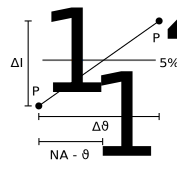
\includegraphics[width=160mm]{drawing.pdf}
    \caption{Schema dell'impianto da vuoto.}
    \label{fig:schema}
\end{figure}

\section{Esecuzione}

L'impianto realizzato è schematizzato in figura \ref{fig:schema}. I vacuometri pirani sono stati disposti
immediatamente ai capi del tubo. Indicheremo le pressioni ai due capi con $P_1$ e $P_2$, come riportato in figura.
La valvola a spillo è stata collocata in fondo all'impianto. È stata mantenuta
aperta la valvola ausiliaria della stessa al fine di evitare problemi con i volumi morti. 

Dopo aver montato l'impianto abbiamo avviato la pompa rotativa, e aspettato di raggiungere il vuoto limite all'interno
del tubo. Per fare ciò abbiamo monitorato al PC l'andamento della pressione al capo $P_2$, assicurandoci che la pressione
si fosse stabilizzata prima di aprire la valvola micrometrica.

Una volta raggiunta la pressione limite abbiamo aperto la valvola micrometrica ad un valore per il quale ci fosse noto
il flusso in entrata. La valvola a spillo è stata tarata nelle esperienze precedenti. A questo punto abbiamo di nuovo
atteso che la pressione si stabilizzasse, prima di misurare la pressione ai capi. 

La procedura è stata ripetuta per 0, 4, 5, 6, 7, 8 giri di apertura della valvola a spillo per ciascuno dei
tubi in esame. Inoltre, per ogni tubo, abbiamo misurato le pressioni aumentando man mano l'apertura della valvola
a spillo per poi misurarle nuovamente chiudendola fino a tornare al valore iniziale.

Durante la sessione di laboratorio abbiamo registrato delle condizioni atmosferiche stabili: $P\ped{atm} = 981 \pm 1$ hPa,
$T = 296 \pm 1 \, \si{\kelvin}$. Entrambe le misure riportano incertezze di risoluzione.

\section{Analisi dati}

Vogliamo ora calcolare i valori di conduttanza dei tubi. Poiché abbiamo registrato due volte le pressioni per ogni valore
di apertura della valvola (una salendo ed una scendendo), dobbiamo prima fare la media tra questi due dati per ottenere
un unico valore di pressione:

\begin{equation}
    P_1 = \frac{P\ped{1,salita} + P\ped{1,discesa}}{2} \qquad P_2 = \frac{P\ped{2,salita} + P\ped{2,discesa}}{2}
\end{equation}

Ora disponiamo, per ciascun tubo e per ciascun valore di apertura della valvola, delle pressioni ai capi del tubo.
A noi interessa la differenza di pressione $\Delta P = P_2 - P_1$, che possiamo usare per calcolare la conduttanza:

\begin{equation}
    C = \frac{Q}{\Delta P}
\end{equation}

I risultati sono riportati nelle tabelle in fondo alla sezione di analisi dati.\\
Dopo aver ottenuto le conduttanze, vogliamo confrontare i valori ricavati con i valori teorici.
Per ottenere i valori teorici dobbiamo essere a conoscenza del tipo di regime di flusso in cui è stato svolto l'esperimento,
poichè le formule che permettono di calcolare la conduttanza sono differenti per i diversi regimi di flusso.
A questo fine calcoliamo il \emph{numero di Knudsen}, o meglio un indicatore equivalente che risulta più comodo da
ottenere con i dati in nostro possesso. L'indicatore è il prodotto $\bar{P}d$, dove $\bar{P}$ è la pressione media misurata nel
tubo e $d$ è il diametro del tubo. Questo indicatore discrimina i regimi di flusso secondo la seguente tabella.

\begin{center}
    \small
    \begin{tabular}{l c c}
        \toprule
        Regime & Tipo di vuoto & $\bar{P} d \; [\si{\pascal\metre}]$ \\
        \midrule
        Viscoso & Basso & $\bar{P} d > 0.6$ \\
        Transitorio & Medio & $1.3\cdot10^{-2} \le \bar{P} d \le 0.6$ \\
        Molecolare & Alto & $\bar{P} d < 1.3\cdot10^{-2}$ \\
        \bottomrule
    \end{tabular}
\end{center}

Per calcolare l'indicatore ci serve $\bar{P}$, che si ottiene con una semplice operazione di media:

\begin{equation}
    \bar{P} = \frac{P_1 + P_2}{2}
\end{equation}

Calcolando l'indicatore per ogni tubo e per ogni apertura della valvola, abbiamo scoperto che gran parte
del nostro esperimento si è svolto in regime transitorio ed in regime viscoso, mentre in neanche un caso abbiamo
lavorato in regime molecolare. I valori di $\bar{P}d$ sono riportati nelle tabelle in fondo a questa sezione,
assieme agli altri dati. Le conduttanze si possono calcolare teoricamente per il regime molecolare e quello
viscoso laminare, mentre per quello transitorio non esiste una formula esplicita. Ci aspettiamo quindi che le nostre
conduttanze siano una via di mezzo tra quelle teoriche per i due casi.

Prima di passare ai calcoli teorici, dobbiamo però verificare che i flussi in camera siano stati laminari nel
caso in cui il sistema fosse in regime viscoso.
A questo fine usiamo il \emph{numero di Reynolds}, che per un tubo è definito come segue:

\begin{equation}
    R_e = \frac{4 M Q}{\pi \eta d R T}
\end{equation}
%
dove $M$ è la massa molare del gas, $Q$ il flusso, $\eta$ la viscosità\footnote{ per calcolare la viscosità dell'aria
alla temperatura del laboratorio abbiamo usato un calcolatore online, reperibile alla pagina http://www.lmnoeng.com/Flow/GasViscosity.htm.
Il calcolatore ignora il fatto che la pressione in camera non è quella atmosferica. Tuttavia il coefficiente di viscosità
dipende solo debolemente dalla pressione e quindi trascuriamo l'effetto della pressione.},
$d$ il diametro della canalizzazione, $R$ la constante dei gas perfetti e $T$ la temperatura.
Sapendo che in base al valore assunto dal numero di Reynolds il regime di flusso viscoso si suddivide in queste tre categorie

\begin{center}
    \small
    \begin{tabular}{l c c}
        \toprule
        Regime & Numero di Reynolds \\
        \midrule
        Viscoso laminare & $R_e < 1200$ \\
        Viscoso intermedio & $1200 < R_e < 2200$ \\
        Viscoso turbolento & $R_e > 2200$ \\
        \bottomrule
    \end{tabular}
\end{center}

e ricordando che il numero di Reynolds dipende solo dal diametro del tubo e dal flusso e non dalla lunghezza o dalle pressioni ai capi,
possiamo classificare il regime di flusso viscoso nel quale abbiamo svolto l'esperienza.
Otteniamo quindi soltanto 10 valori del numero di Reynolds (i dati sono misurati in \si{\kg\per\m\per\s}):

\begin{center}
    \small
    \begin{tabular}{l c c}
        \toprule
        \multirow{2}*{Nr. giri} & \multicolumn{2}{c}{Diametro} \\
         & 4 mm & 2.5 mm \\
        \midrule
        4 & $(2.433 \pm 0.004) \cdot 10^{-2}$ & $(3.893 \pm 0.006) \cdot 10^{-2}$ \\
        5 & $(1.196 \pm 0.001) \cdot 10^{-1}$ & $(1.914 \pm 0.002) \cdot 10^{-1}$  \\
        6 & $1.115 \pm 0.002$ &                 $1.784 \pm 0.003$                 \\
        7 & $12.57 \pm 0.02$ &                  $20.11 \pm 0.04$                  \\
        8 & $79.1 \pm 0.2$ &                    $126.5 \pm 0.2$                   \\
        \bottomrule
    \end{tabular}
\end{center}

Quindi in tutti i casi il sistema ha lavorato in regime laminare. Possiamo applicare le formule per il calcolo
teorico della conduttanza, al fine di confrontarle con i nostri dati.

Assumendo un regime molecolare, si può calcolare che per un tubo di diametro $d$ e lunghezza $l$, la conduttanza vale:

\begin{equation}
    C\ped{mol} = 120 \frac{d^3}{l}
\end{equation}

Si ottengono 4 diversi valori della conduttanza, uno per ogni tubo. I valori calcolati con questa formula
sono riportati nella seguente tabella.

\begin{center}
    \small
    \begin{tabular}{c c c c}
        \toprule
        8000x4 & 800x4 & 8000x2.5 & 800x2.5 \\
        \midrule
        $9.6 \cdot 10^{-7}$ & $9.6 \cdot 10^{-6}$ & $2.34 \cdot 10^{-7}$ & $2.34 \cdot 10^{-6}$ \\
        \bottomrule
    \end{tabular}
\end{center}

Nel caso di regime viscoso laminare, si può invece dimostrare che la conduttanza dipende anche dalla pressione media
$\bar{P}$ (già introdotta sopra per calcolare l'indicatore $\bar{P}d$):

\begin{equation}
    C\ped{lam} = 1350 \frac{\bar{P} d^4}{l}
\end{equation}

Poiché le conduttanze teoriche in regime viscoso laminare dipendono dalla pressione esse variano al variare del tubo 
e al variare del flusso in ingresso. I valori di $C\ped{lam}$ sono elencati nelle seguenti tabelle che includono anche
tutti gli altri dati calcolati sopra.

\paragraph{Tubo 8000x4 \\}
\begin{center}
    \small
    \begin{tabular}{c c c c c}
        \toprule
        Nr. giri & C $\pm$ dC $[\si{\metre^3\s^{-1}}]$ & $\bar{P}d$ $[\si{\Pa\meter}]$ & Regime & (C\ped{lam} $\pm$ dC\ped{lam}) $[\si{\metre^3\s^{-1}}]$ \\
        \midrule
        4 & $(7 \pm 1) \cdot 10^{-7}$ & 0.38 & Transitorio & $(4.1 \pm 0.6) \cdot 10^{-6}$ \\
        5 & $(2.6 \pm 0.4) \cdot 10^{-6}$ & 0.47 & Transitorio & $(5.1 \pm 0.7) \cdot 10^{-6}$ \\
        6 & $(1.0 \pm 0.2) \cdot 10^{-5}$ & 1.1 & Viscoso & $(1.2 \pm 0.2) \cdot 10^{-5}$ \\
        7 & $(3.4 \pm 0.5) \cdot 10^{-5}$ & 3.9 & Viscoso & $(4.3 \pm 0.6) \cdot 10^{-5}$ \\
        8 & $(9 \pm 1) \cdot 10^{-5}$ & 10 & Viscoso & $(1.0 \pm 0.1) \cdot 10^{-4}$  \\
        \bottomrule
    \end{tabular}
\end{center}

%% attenzione qui tabelle di prova
%\paragraph{Tubo 8000x4 VERSIONE 2\\}
%\begin{center}
%    \small
%    \begin{tabular}{c c c c c c}
%        \toprule
%        Nr. giri & C $[\si{\metre^3\s^{-1}}]$ & dC $[\si{\metre^3\s^{-1}}]$ & Regime & C\ped{teorica} $[\si{\metre^3\s^{-1}}]$ & dC\ped{teorica} $[\si{\metre^3\s^{-1}}]$ \\
%        \midrule
%        4 & $6.6372 \cdot 10^{-7}$ & $1 \cdot 10^{-7}$ & Transitorio & $4.0867 \cdot 10^{-6}$ & $6 \cdot 10^{-7}$ \\
%        5 & $2.6187 \cdot 10^{-6}$ & $4 \cdot 10^{-7}$ & Transitorio & $5.0695 \cdot 10^{-6}$ & $7 \cdot 10^{-7}$ \\
%        6 & $1.0252 \cdot 10^{-5}$ & $1 \cdot 10^{-6}$ & Viscoso & $1.2172 \cdot 10^{-5}$ & $2 \cdot 10^{-6}$ \\
%        7 & $3.3973 \cdot 10^{-5}$ & $5 \cdot 10^{-6}$ & Viscoso & $4.2660 \cdot 10^{-5}$ & $6 \cdot 10^{-6}$ \\
%        8 & $8.9041 \cdot 10^{-5}$ & $1 \cdot 10^{-5}$ & Viscoso & $1.1275 \cdot 10^{-4}$ & $1 \cdot 10^{-5}$  \\
%        \bottomrule
%    \end{tabular}
%\end{center}
%% attenzione qui tabelle di prova

\paragraph{Tubo 800x4 \\}
\begin{center}
    \small
    \begin{tabular}{c c c c c}
        \toprule
        Nr. giri & C $\pm$ dC $[\si{\metre^3\s^{-1}}]$ & $\bar{P}d$ $[\si{\Pa\meter}]$ & Regime & C\ped{lam} $\pm$ dC\ped{lam} $[\si{\metre^3\s^{-1}}]$ \\
        \midrule
        4 & $(4.5 \pm 0.7) \cdot 10^{-6}$ & 0.061 & Transitorio & $(7 \pm 1) \cdot 10^{-6}$ \\
        5 & $(1.4 \pm 0.2) \cdot 10^{-5}$ & 0.093 & Transitorio & $(1.0 \pm 0.1) \cdot 10^{-5}$ \\
        6 & $(3.9 \pm 0.6) \cdot 10^{-5}$ & 0.32 & Transitorio & $(3.5 \pm 0.5) \cdot 10^{-5}$ \\
        7 & $(1.5 \pm 0.2) \cdot 10^{-4}$ & 1.1 & Viscoso & $(1.2 \pm 0.2) \cdot 10^{-4}$ \\
        8 & $(3.5 \pm 0.7) \cdot 10^{-4}$ & 3.8 & Viscoso & $(4.1 \pm 0.5) \cdot 10^{-4}$ \\
        \bottomrule
    \end{tabular}
\end{center}

\paragraph{Tubo 8000x2.5 \\}
\begin{center}
    \small
    \begin{tabular}{c c c c c}
        \toprule
        Nr. giri & C $\pm$ dC $[\si{\metre^3\s^{-1}}]$ & $\bar{P}d$ $[\si{\Pa\meter}]$ & Regime & C\ped{lam} $\pm$ dC\ped{lam} $[\si{\metre^3\s^{-1}}]$ \\
        \midrule
        4 & $(3.2 \pm 0.5) \cdot 10^{-7}$ & 0.48 & Transitorio &  $(1.3 \pm 0.2) \cdot 10^{-6}$ \\
        5 & $(1.2 \pm 0.2) \cdot 10^{-6}$ & 0.65 & Viscoso & $(1.7 \pm 0.2) \cdot 10^{-6}$ \\
        6 & $(4.0 \pm 0.6) \cdot 10^{-6}$ & 1.8 & Viscoso & $(4.7 \pm 0.7) \cdot 10^{-6}$ \\
        7 & $(1.5 \pm 0.2) \cdot 10^{-5}$ & 5.3 & Viscoso & $(1.4 \pm 0.2) \cdot 10^{-5}$ \\
        8 & $(1.5 \pm 0.2) \cdot 10^{-5}$ & 34 & Viscoso & $(9 \pm 1) \cdot 10^{-5}$ \\
        \bottomrule
    \end{tabular}
\end{center}
%WTF! gli ultimi due valori sono praticamente uguali... sarà corretto? mah! chi mai lo saprà?% per altro è l'unico valore di viscoso che non torna...

\paragraph{Tubo 800x2.5 \\} 
\begin{center}
    \small
    \begin{tabular}{c c c c c}
        \toprule
        Nr. giri & C $\pm$ dC $[\si{\metre^3\s^{-1}}]$ & $\bar{P}d$ $[\si{\Pa\meter}]$ & Regime & C\ped{lam} $\pm$ dC\ped{lam} $[\si{\metre^3\s^{-1}}]$ \\
        \midrule
        4 & $(2.0 \pm 0.3) \cdot 10^{-6}$ & 0.09 & Transitorio & $(2.1 \pm 0.3) \cdot 10^{-6}$ \\
        5 & $(5.0 \pm 0.7) \cdot 10^{-6}$ & 0.15 & Transitorio & $(4.0 \pm 0.6) \cdot 10^{-6}$ \\
        6 & $(1.5 \pm 0.2) \cdot 10^{-5}$ & 0.49 & Transitorio & $(1.3 \pm 0.2) \cdot 10^{-5}$ \\
        7 & $(4.7 \pm 0.7) \cdot 10^{-5}$ & 1.8 & Viscoso & $(4.9 \pm 0.7) \cdot 10^{-5}$ \\
        8 & $(1.3 \pm 0.2) \cdot 10^{-4}$ & 4.8 & Viscoso & $(1.3 \pm 0.2) \cdot 10^{-4}$ \\
        \bottomrule
    \end{tabular}
\end{center}

%la compatibilità è FFTTT FFTTT FFTTF TTTTT (F = False; T = True)

In base ai dati da noi ottenuti possiamo notare come i valori della conduttanza corrispondenti a 4, 5 giri della valvola a spillo siano praticamente sempre incompatibili con i relativi valori teorici. Questo è dovuto al fatto che il regime di flusso in queste situazioni non era viscoso, bensì transitorio. Inoltre, non siamo a conoscenza di alcuna formula specifica che descriva correttamente la conduttanza in condizioni di regime transitorio.
Per quanto riguarda i dati ricavati con i giri più alti della valvola  aspillo (6, 7 e 8) il regime diventa nella maggiorparte dei casi viscoso ed essendo nelle condizioni di flusso viscoso laminare, descritte dal numero di Reynolds, abbiamo potuto calcolare la conduttanza teorica. I valori ricavati empiricamente sono risultati compatibili con quelli ricavati teoricamente. % ad eccetto del valore del tubo 8000x2.5 a 8 giri, il quale è fuori con un poggiuolo. :D

% la domanda comunque rimane: come abbiamo calcolato la conduttanza per i valori in condizione di regime transitorio? domani me lo spiegate, nè sì? thanks